\subsubsection{项目背景}
\showprojectlocation位于滨江大道和经三路交叉口西南片,远期占地约210亩,根据《城北污水处理厂初步设计说明书》其远期污水处理服务范围是针对循环经济试验园72家企业进行工业废水处理。根据项目批复和建设计划近期(2010年)处理规模8万m³/d,远期(2020年)日处理规模16万m³/d。近期工程分两个阶段实施,第一阶段实施4万m³/d,第二阶段实施4万m³/d规模。第一阶段实际竣工时间为2015年9月,目前厂区实际进水量约为15000m³/d,还未开始第二阶段建设实施。\par
园区内有7家企业的工业废水多年以来一直由企业自行处理达到一定的标准经由二冶大沟排入长江,目前政府正对其排污管网进行改造,预计在2017年11月30日完成,改造完成以后,其工业废水即将纳入城北污水处理厂。此部分废水非城北污水处理厂一期一阶段工程设计的设计范围,为确保改造后污水厂出水达标排放,需要对该厂进行设计改造。其中包括的铜陵泰富排放的焦化废水生化性差、盐度、色度高,需要重点关注。\par
其二,根据《“十三五”重点流域水环境综合治理建设规划》要求,园区内工业企业排水必须经过园区内集中污水厂处理后才能排入环境水体,不允许自行处理直接排放,同时,城北污水厂原设计出水水质执行《城镇污水处理厂污染物排放标准》(GB18918-2002)中的一级B标准已经不能满足国家现行标准要求,需要提高至一级A标准。\par
铜陵城北污水处理厂近期处理规模8万m³/d,远期处理规模16万m³/d。近期工程分两个阶段实施,第一阶段实施4万m³/d,第二阶段实施4万m³/d规模,已建成近期一阶段处理规模4万m³/d。\par
提标改造工程在已建成的近期一阶段工程基础上实施,建设规模为4万m³/d。\par
\subsubsection{项目工艺介绍}
改造后项目工艺流程如下图所示:\par
{
    \centering 
    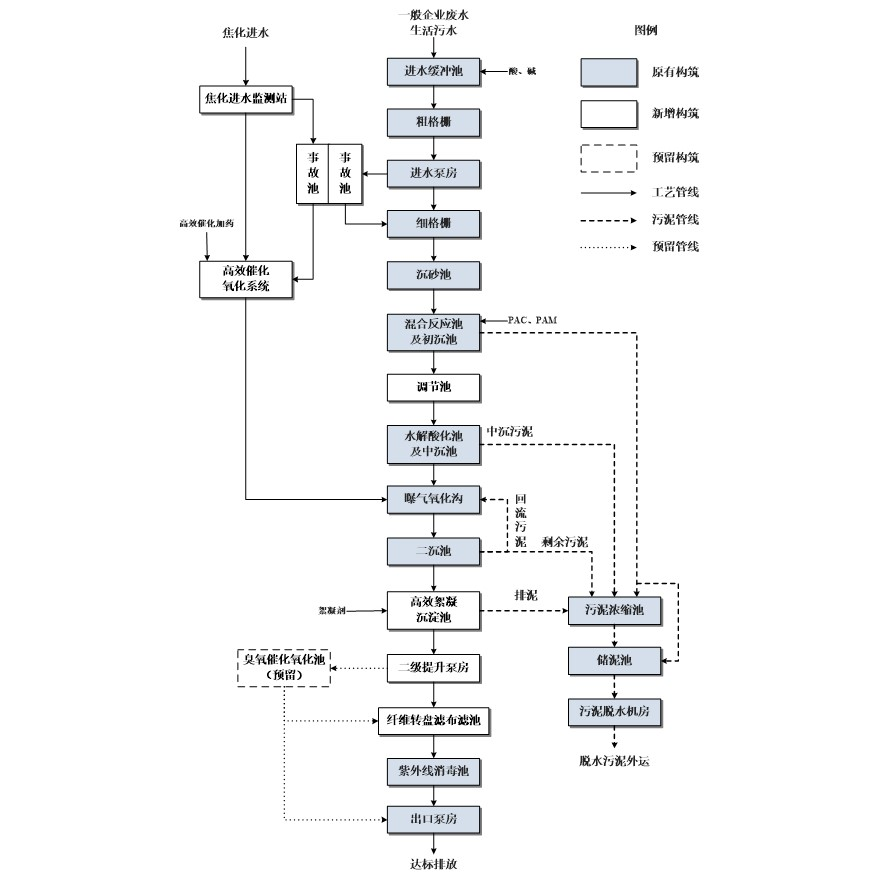
\includegraphics[width=150mm]{Img/fig3.jpg}
    \captionof{figure}{项目改造工艺流程}
    \label{fig3}
}\par
焦化进水经过进水监测站后进入高效催化氧化系统预处理,之后与处理过的一般企业废水混合。一般企业废水进入进水缓冲池,经过粗格栅被提升至细格栅沉砂池、初沉池后进入调节池配水进行水解酸化,之后与处理过的焦化水混合,由曝气氧化沟生化处理,经二沉池高校絮凝沉淀池、滤布滤池后紫外消毒并外排。\par
其中高效催化氧化工艺是本项目自研的一体化装置,依据Fenton反应原研发出的集电化学混凝、催化氧化及絮凝沉淀于一体的优良工艺。与传统Fenton处理工艺相比,高效催化氧化工艺对pH值的要求更低,pH在3-8范围内均可发生反应,基本不用调节pH。以高效催化氧化反应器(成套设备)代替调酸池、催化氧化反应塔、脱气池、调碱池等单体构筑,采用全程自动化控制,工艺更紧凑、运行维护更简便。
以氧化絮凝池代替絮凝反应池,采用先进的多次氧化机理,利用弱氧化剂进一步氧化,提高氧化处理效果。\par

\subsubsection{焦化废水处理工艺设计} 
A. 焦化进水监测站
(1)构筑物功能	\par 
在线检测焦化废水进水水质,设计规模3500m³/d。主要检测指标:pH、CODCr、氨氮、硫化物。\par 
结构形式:构筑物为半地下钢砼结构,建筑物为框架结构。\par 
(2)建(构)筑物				\par 
焦化进水监测站:6×4.5m;1座;	\par 
焦化缓冲池:6×4.5×4.5m;1座。	\par 
(3)配套主要设备				\par 
1)pH在线监测仪	\par 
数量:1套;\par 
参数:测量范围0~14;精度0.1;\par 
2)COD在线监测仪	\par 
数量:1套;\par 
3)氨氮在线监测仪	\par 
数量:1套;\par 
4)硫化物在线监测仪	\par 
数量:1套;\par 
5)电磁流量计	\par 
数量:1台;\par 
参数:DN250,PN1.0.\par 
6)对夹式电动蝶阀	\par 
数量:2台;\par 
参数:DN250,PN1.0。\par 
7)轴流风机	\par 
数量:1台;\par 
参数:Q=1224m³//h,α=15°,P=155KPa,N=0.12kW。\par 
8)提升泵	\par 
数量:2台,离心泵,1用1备;\par 
参数:Q=146.0m³/h,H=17.0m,N=15.0kw。\par 
9)电动葫芦:配套滑触线、配套开关等;\par 
数量:1台;\par 
参数:CD1型,T=1t,H=9m,N=1.7KW,轨道长6m。\par 
B. 高效催化氧化系统 
(1)构筑物功能:\par 
在催化剂作用下,利用铁盐、双氧水等强氧化剂氧化降解水中难降解有机物,使出水COD达到排放标准,并通过絮凝沉淀去除水中大部分SS、TP等污染物。\par 
设计规模3500m³/d,仅处理铜陵泰富(焦化厂)排水,出水进入氧化沟,进一步去除废水中的氨氮和总氮处理。\par 
(2)结构形式:构筑物为半地下钢砼结构,建筑物为框架结构;\par 
(3)设计参数:\par 
设计规模:Q=3500m³/d;\par 
氧化接触时间:HRT=0.5hr\par 
(4)建(构)筑物:\par 
氧化絮凝池:7.0×6.0×4.5m;1座	;\par 
氧化沉淀池:D16×3.5m;1座	;\par 
鼓风机房:6.0×4.0m;1座	。\par 
(5)配套设备	\par 
1)高效催化氧化反应器	\par 
数量:1套;\par 
参数:2205双相不锈钢材质。\par 
2)专用曝气管	\par 
数量:1套;\par 
参数:ABS材质。\par 
3)罗茨风机	\par 
数量:2台,1用1备;\par 
参数:Q=11.2m³/min,H=49.0kpa,N=15.0kw。\par 
4)电动葫芦	\par 
数量:1套;\par 
参数:T=2t,H=6m,N=3.4kW,导轨长6m。\par 
5)单周边式刮泥机	\par 
数量:1套;\par 
参数:D=16m,N=1.1kw。\par 
6)无堵塞排泥泵	\par 
数量:2台,1用1备;\par 
参数:Q=30m³/h,H=20m, N=5.5kw。\par 
C. 加药间 
(1)构筑物功能	\par 
布置加药设备,为高效絮凝沉淀池和高效催化氧化提供药液。\par 
(2)结构形式:构筑物为钢砼结构,建筑物为框架结构;\par 
(3)建(构)筑物:				\par 
加药间:30×16m;1座;	\par 
溶药池:2.5×2.5×4.0m;2座;加药间内;\par 
储药池:2.5×2.5×4.0m;2座;加药间内.\par 
(4)配套设备	\par 
1)特殊混凝剂溶药罐	\par 
数量:3套,2用1备;\par 
参数:V=3.0m,φ1600X2080mm,N=1.1kW。\par 
2)特殊混凝剂加药计量泵	\par 
数量:3套,2用1备;\par 
参数:Q=500L/h,5bar,N=0.25kW。\par 
3)絮凝剂制备系统PAM-	\par 
数量:1套;\par 
参数:N=0.75kW,投加能力1000L/h,配置浓度0.1\%。\par 
4)PAM-加药螺杆泵	\par 
数量:2台,1用1备,变频调速;\par 
参数:Q=1000L/h,P=0.3MPa,N=1.1kW。\par 
5)PAM加药螺杆泵	\par 
数量:2台,1用1备;\par 
参数:Q=2.0m³/h,H=20m,1.1kW。\par 
6)硫酸亚铁加药系统	\par 
数量:1套;\par 
参数:含药液提升泵、加药泵、搅拌器、超声液位计等。\par 
7)双氧水加药系统	\par 
数量:1套;\par 
参数:含药液提升泵、加药泵、搅拌器、超声液位计等。\par 
8)液碱加药系统	\par 
数量:1套;\par 
参数:含储药罐、加药泵、卸料泵、超声液位计等。\par 
9)双氧水自动配药系统	\par 
数量:1套;\par 
参数:含储药罐、加药泵、卸料泵、磁翻板液位计等。\par 
10)硫酸自动配药系统	\par 
数量:1套;\par 
参数:含储药罐、加药泵、卸料泵、磁翻板液位计等。\par 
11)电动葫芦:配套滑触线、配套开关等;\par 
数量:1台;\par 
参数:T=1t,H=9m,N=1.7kW,导轨长40m。\par 
